\begin{figure}[t]
% \makebox[\linewidth][c]{
\centering
\begin{subfigure}{0.49\textwidth}
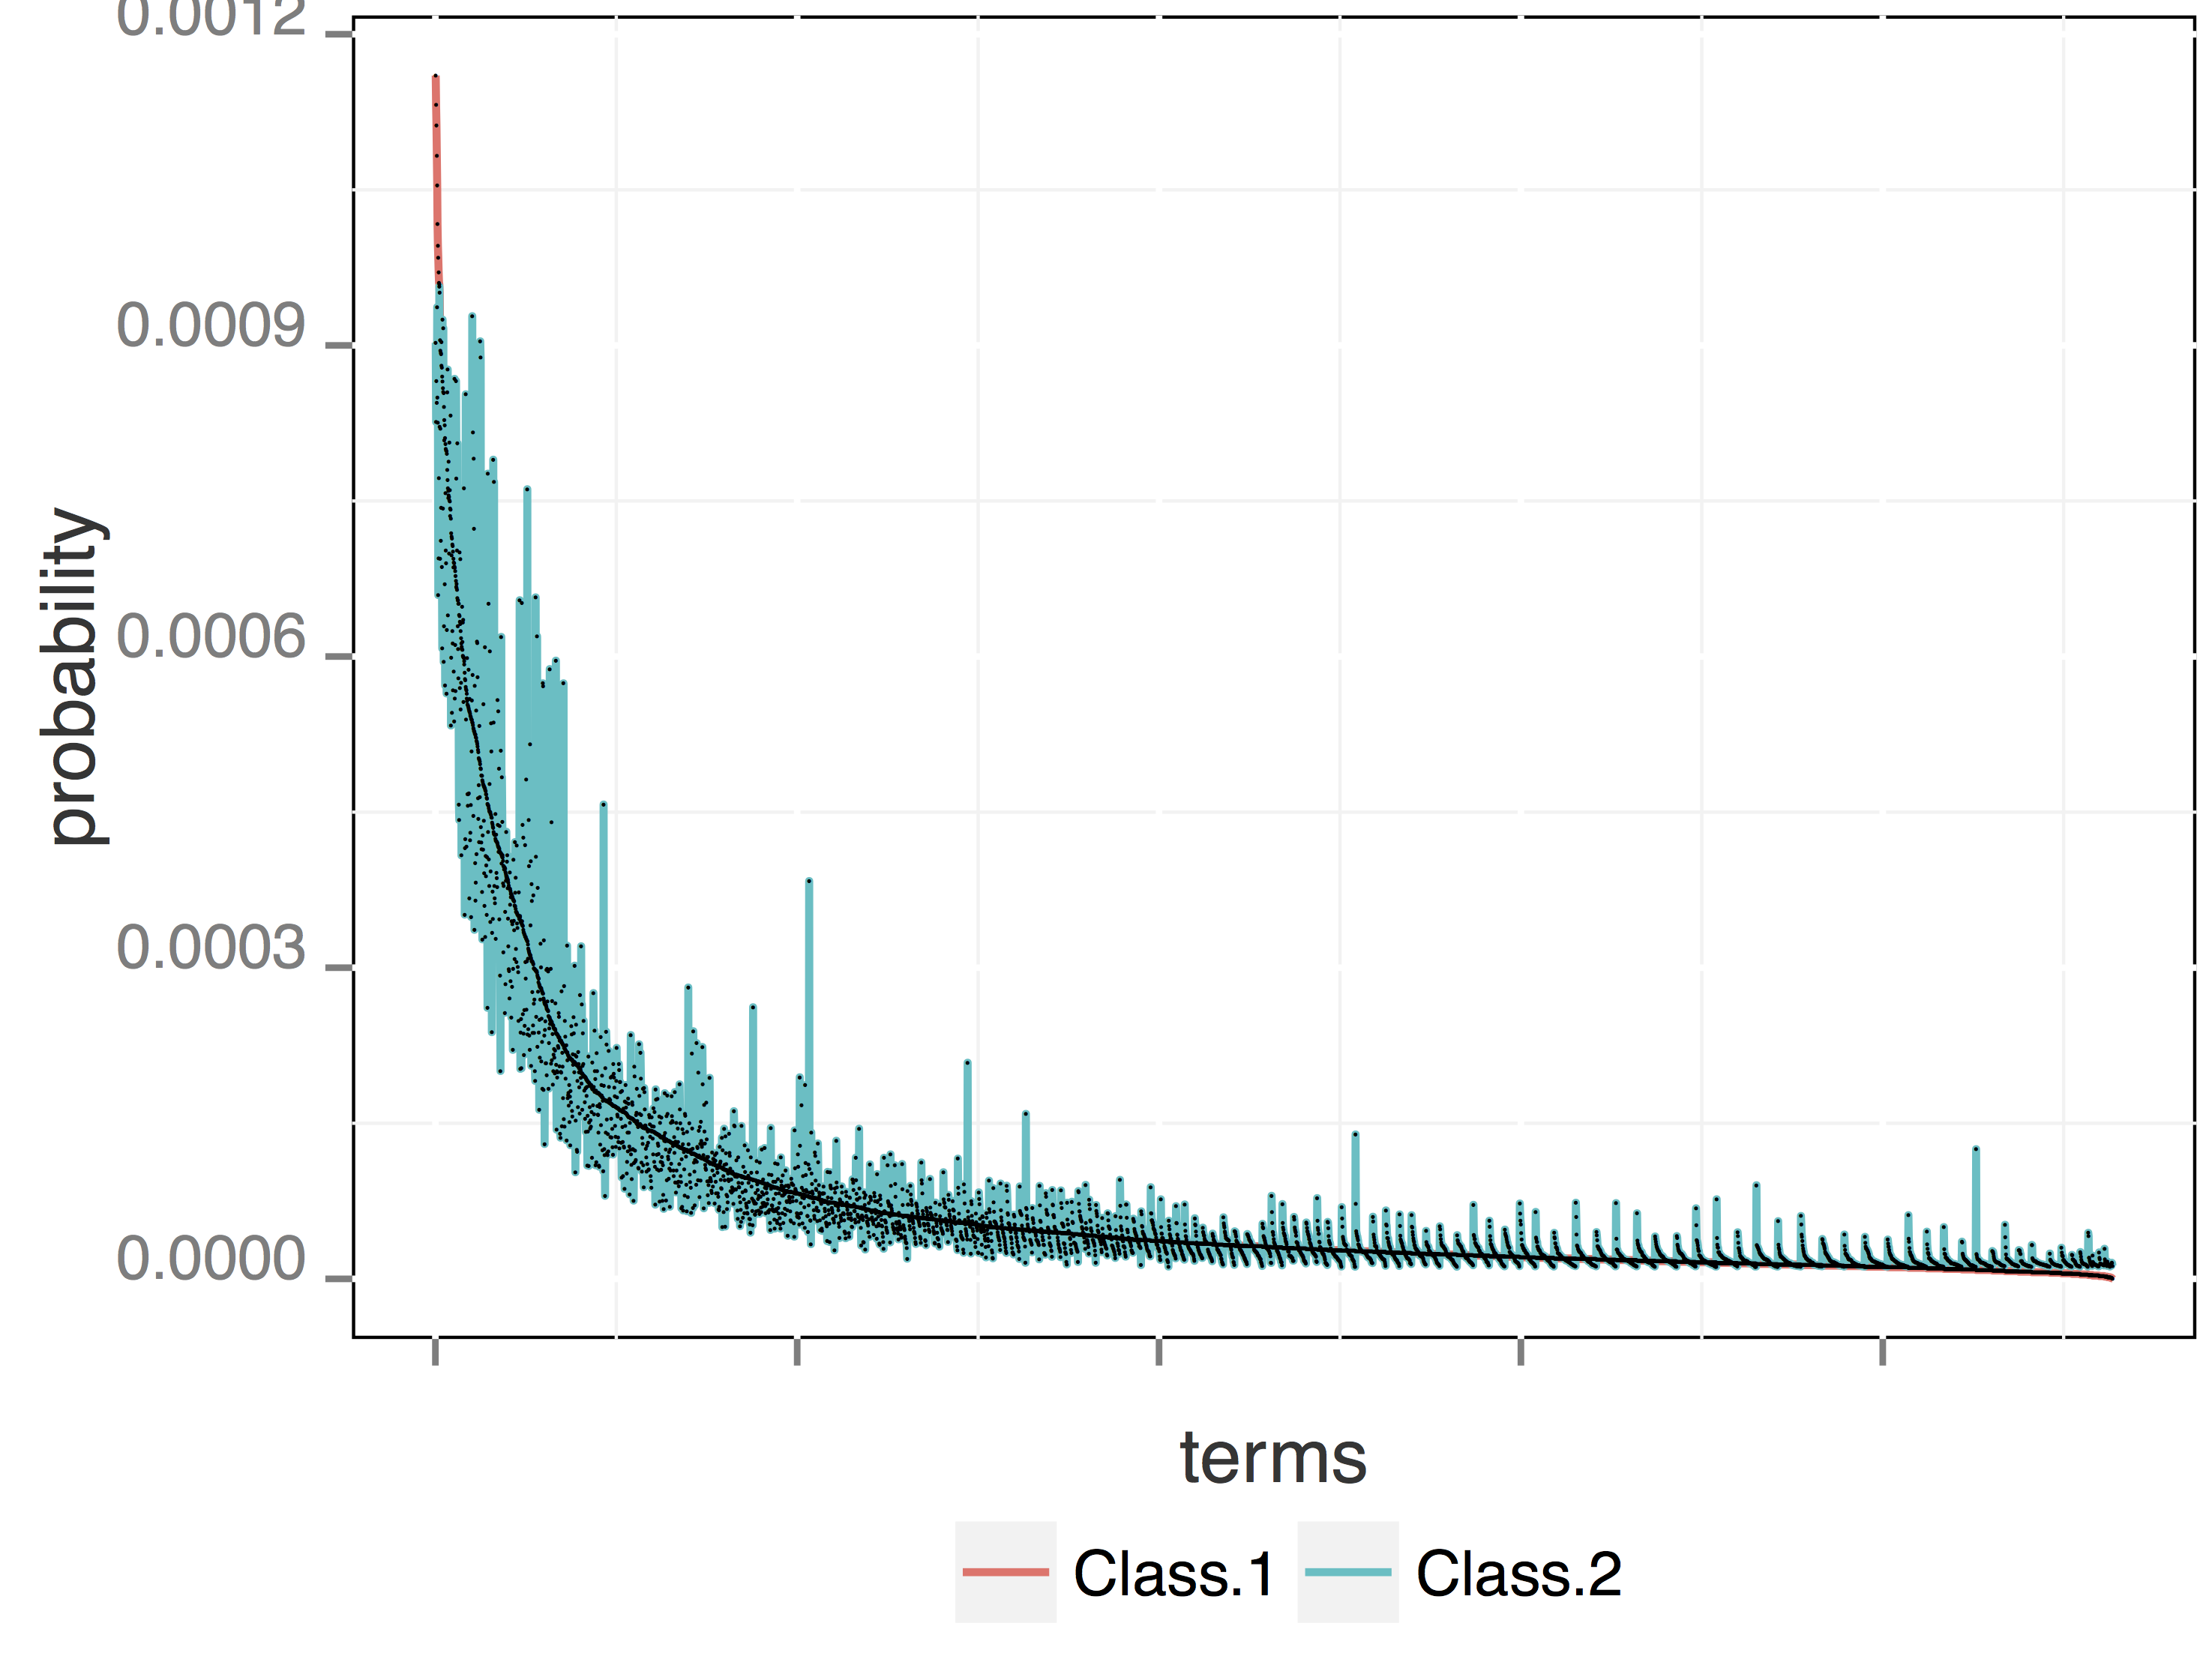
\includegraphics[width=\linewidth]{02-part-01/chapter-03/figs_and_tables/img_example-slm.png}
\caption{\label{fig:sep-slm} \scriptsize{A non-separable representation of data.}}
\end{subfigure}
\hfill
\begin{subfigure}{0.49\textwidth}
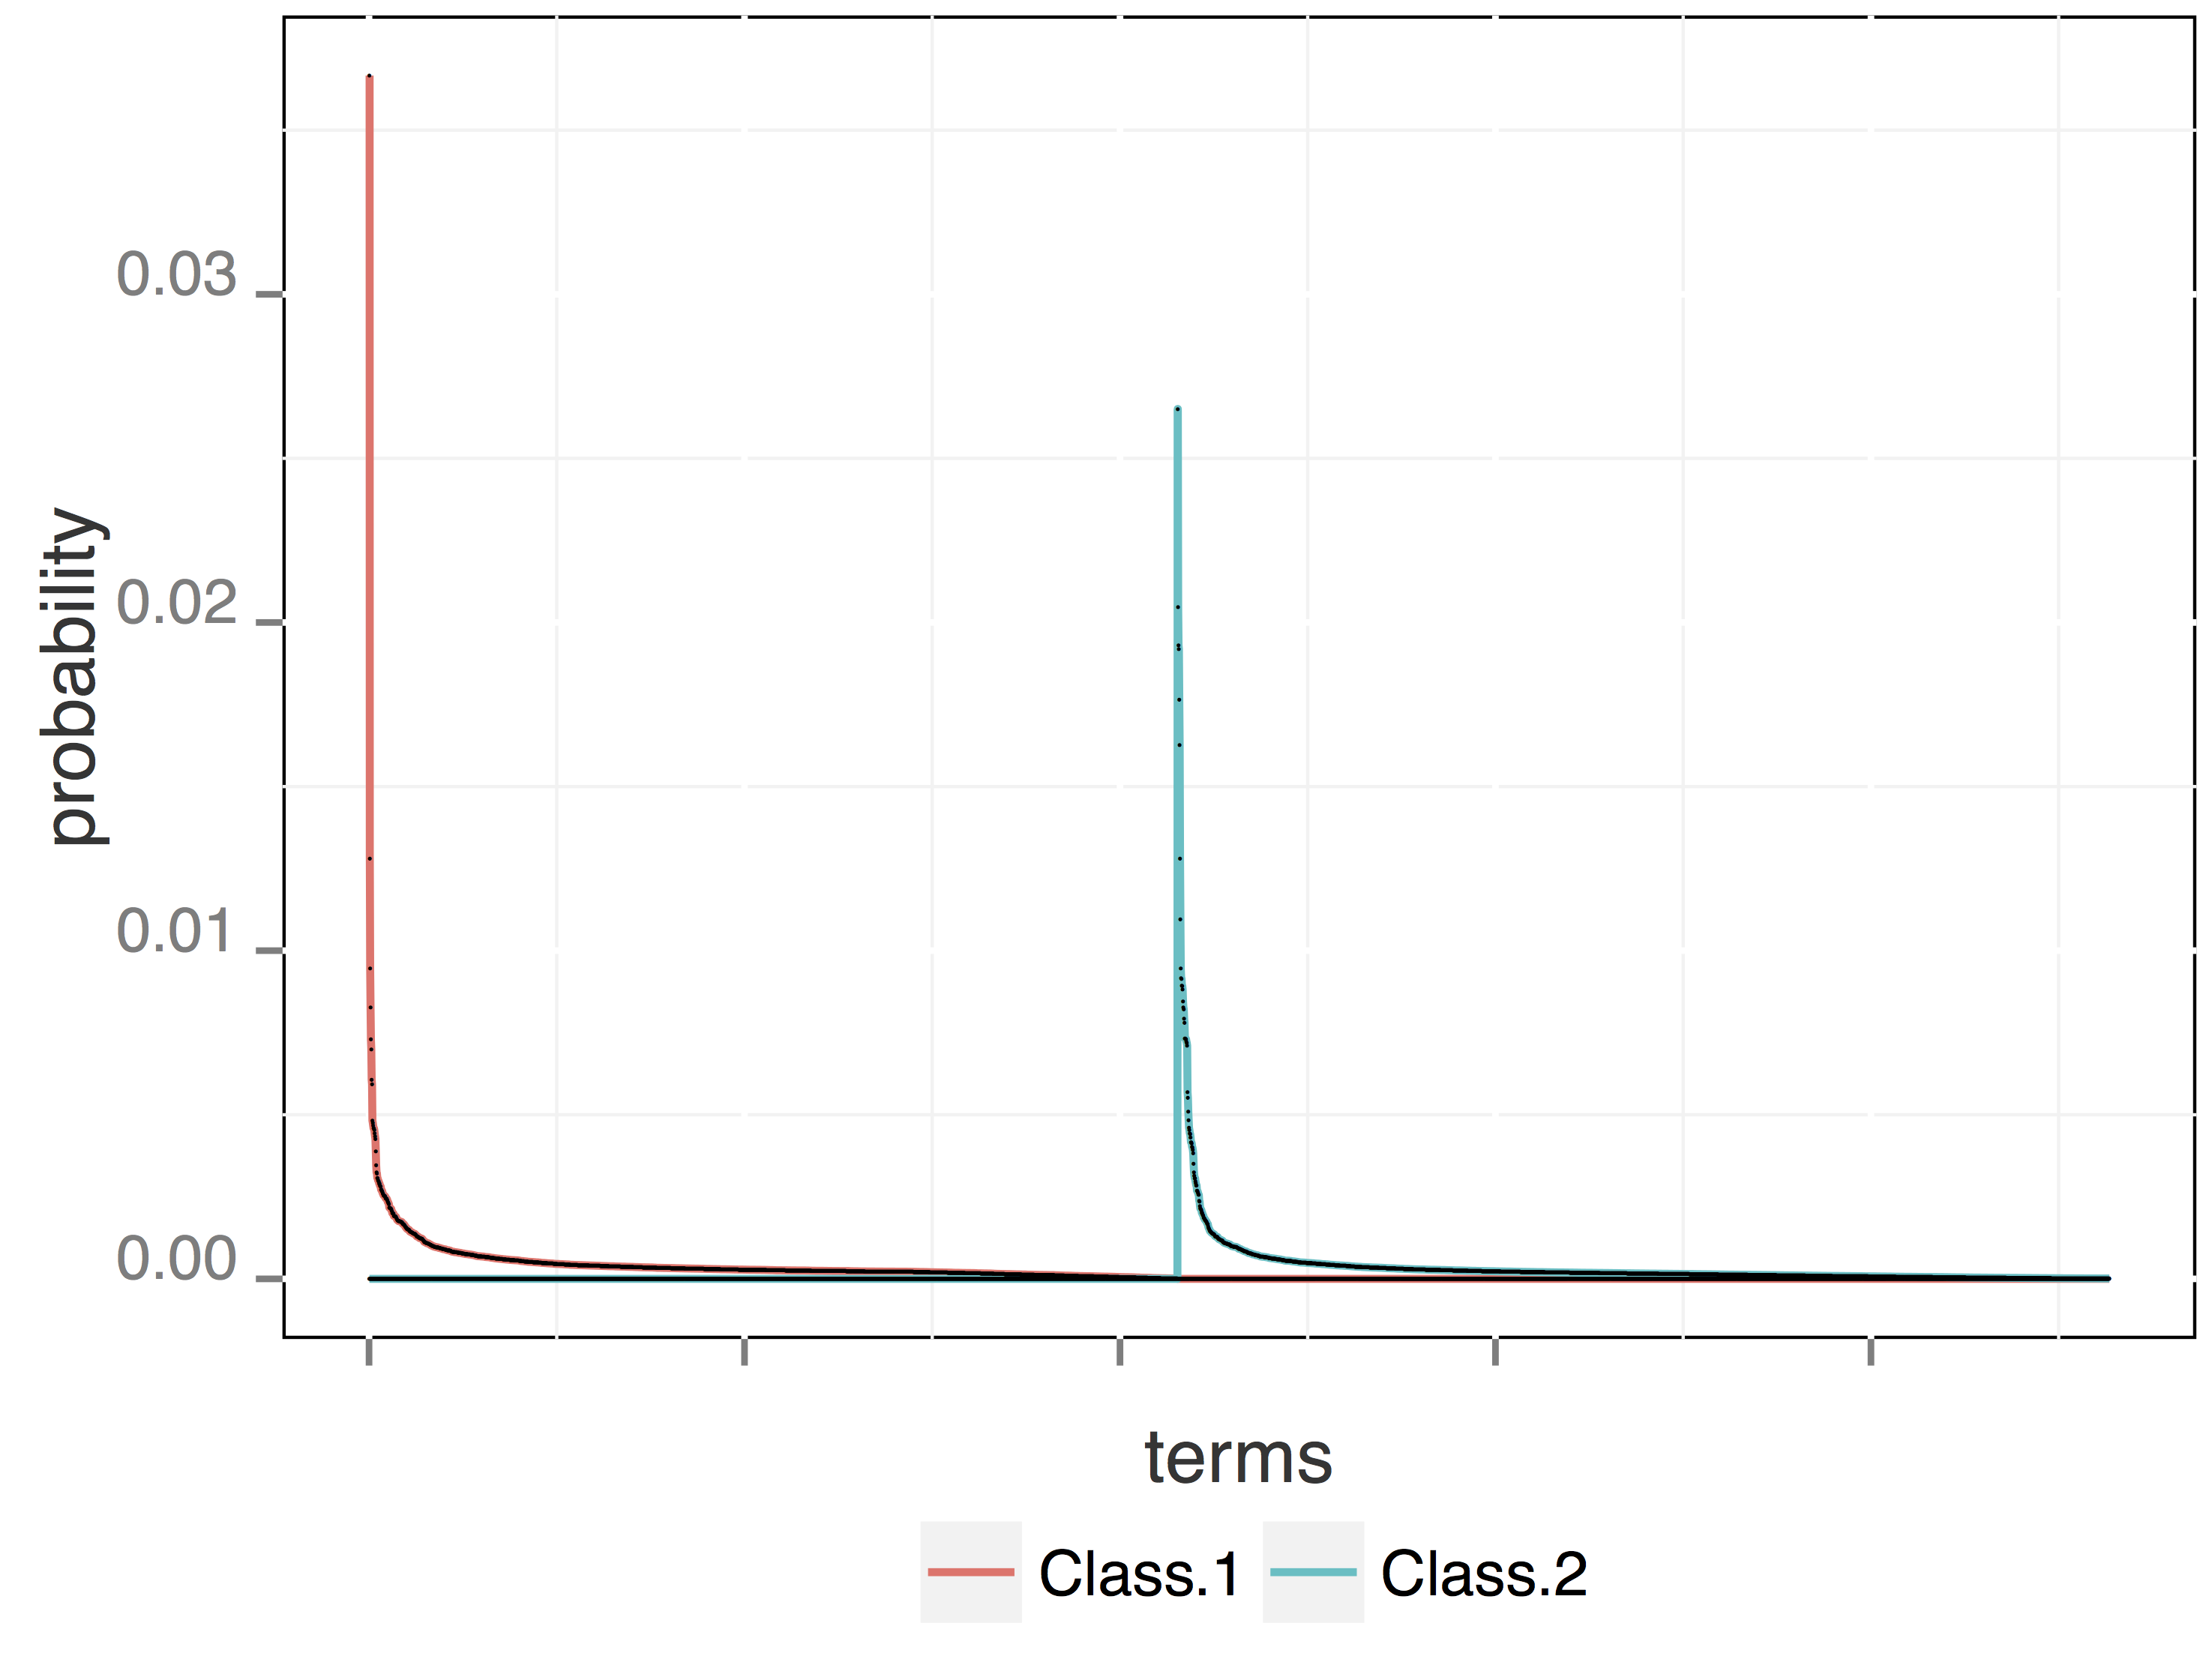
\includegraphics[width=\linewidth]{02-part-01/chapter-03/figs_and_tables/img_example-swlm.png}
\caption{\label{fig:sep-swlm} \scriptsize{A well-separable representation of data}}
\end{subfigure}
\caption{\label{fig:sep_rep} Probability distribution over terms for data in two different classes, (entities in the statues layer of the parliament), sorted based on the term weights in one of the classes.}
% }
\end{figure}